\documentclass[../main.tex]{subfiles}

\begin{document} %%%%%%%%%%%%%%%%%%%%%%%%%%%%%%%%%%%%%%%%%%%%%%%%%%%%%%%%%%%%
\section{La Memoria}
    \subsection{La Abstracción del Espacio de Direcciones: Introducción}
        La memoria física puede ser imaginada como un arreglo de direcciones de memoria una detrás de otra.
        \\
        Esta “abstracción” es manejable mientras la cantidad de memoria necesitada esta en un rango “manejable” y cual es ese rango. En DOS (Disk Operating System) ese rango lo daba la elección de una arquitectura determinada, la del 8086, que permite tener direcciones de memoria de hasta 220
        bits, es decir 1 MegaByte de memoria.

        \begin{figure}[bh]
            \centering
            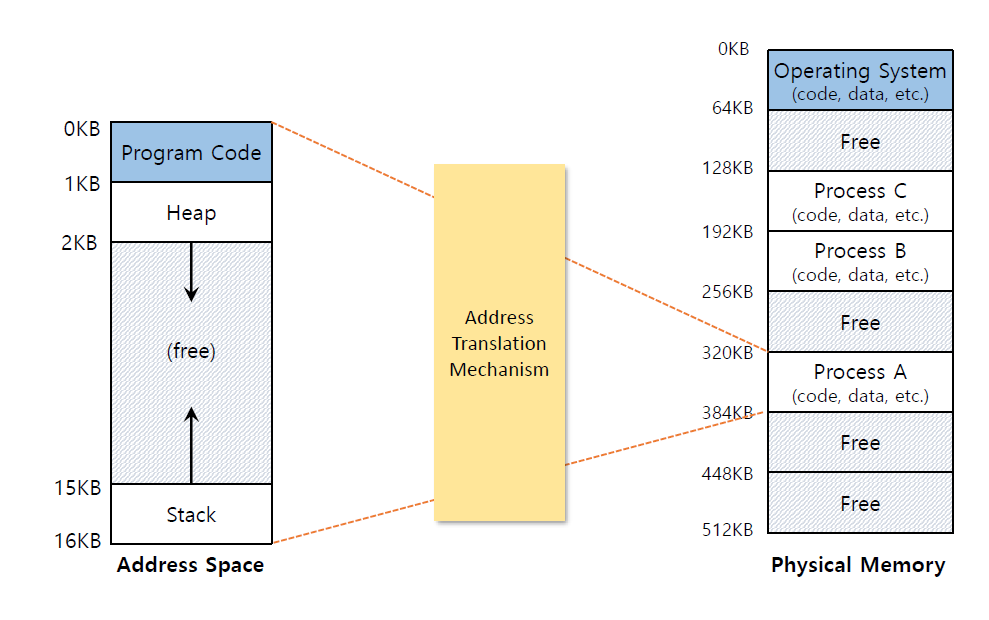
\includegraphics[scale=0.45]{../images/address_traslation_01.png}
            \label{fig:address_traslation_01}
            \caption{Address traslation.}
        \end{figure}

    \subsection{El Espacio de Direcciones o Address Space}
        El Address Space de un proceso contiene todo el estado de la memoria de un programa en ejecución. Es la abstracción para la memoria.\\

        El Espacio de Direcciones o Address Space es la abstracción fundamental sobre la memoria de una computadora. Consiste en dar un mecanismo fácil de usar a lo usuarios de la computadora.

        Cuando se describe el espacio de direcciones se está describiendo la abstracción que el Sistema Operativo le proporciona al programa en ejecución sobre la memoria de la computadora.

        Cuando el Sistema Operativo implementa esta abstracción, se dice que el O.S. está Virtualizando la Memoria ya que el programa en ejecución cree que está cargado en un lugar particular de la memoria (la posición 0 dirección virtual o virtual address) y tiene potencialmente toda la memoria para él.\\
        
        Metas principales de la virtualización es :
        \begin{itemize}
            \item transparencia.
            \item eficiencia: tiempo y espacio.
            \item protección: proteger a los procesos unos de otros como también proteger al sistema operativo de los procesos.
                \begin{itemize}
                    \item aislamiento: cada proceso tiene su propio espacio de direcciones aislado.
                \end{itemize} 
        \end{itemize}

    \subsection{El API de Memoria}
        \subsubsection{Tipos de Memoria}
            \begin{itemize}
                \item \textbf{Memoria de stack:} su reserva y liberación es manejada implícitamente por el compilador en nombre del programador por esta razón a veces también se denomina memoria automática.
                \item \textbf{Memoria de heap:} es la memoria que se reserva y libera explícitamente por el programador.
            \end{itemize}

    \subsection{Address Translation}
        Existen dos puntos importantes a la hora de virtualizar memoria:
        \begin{itemize}
            \item flexibilidad
            \item eficiencia
        \end{itemize}

        Para lograr esto se usa la técnica de \textbf{address translation} o traducción de direcciones (Hardware-Based Address Translation).
    
    \subsection{Hacia una eficiente Address Translation}
        Mecanismos para mejorar el rendimiento de la traducción de las direcciones.\\

        Se usara un \textbf{caché (o escondrijo)}, que consiste en una copia de ciertos datos que pueden ser accedidos mas de una vez más rápidamente.\\

        Uno de los problemas del \textbf{address translation} reside en la \textbf{velocidad de la traducción} para ello se utilizan técnicas que mejoran la velocidad de esta traducción. Se utiliza un mecanismo de hardware llamado \textbf{Translation-Lookaside Buffer}; o tambien conocido como \textbf{TLB}. La TLB es parte de la MMU y es simplemente un mecanismo de cache de las traducciones mas utilizadas entre los pares virtual to physical address. Por ende un mejor nombre para este mecanismo podría ser address translation cache.\\

        Por cada referencia a la memoria virtual, el hardware primero chequea la TLB para ver si esa traducción esta guardada ahí; si es así la traducción se hace rápidamente sin tener que consultar a la page table (la cual tiene todas las traducciones).\\

        Normalmente se chequean todas las entradas de la TLB contra la virtual page, si existe matcheo el procesador utiliza ese matcheo para formar la physical address, ahorrándose todos los pasos de la traducción.

        Cuand existe matcheo TLB hit, cuando del proceso anterior no existe matcheo en la TLB , se dice que se tiene un TLB miss














\end{document}  %%%%%%%%%%%%%%%%%%%%%%%%%%%%%%%%%%%%%%%%%%%%%%%%%%%%%%%%%%%%%